\section{Learning What Task Plan to Refine}
The approach presented thus far can be succinctly described as learning \emph{how} to
refine a single high-level plan. In this section, we present a method for learning
\emph{which} plan to try refining. Recall that in Alg.\,\ref{alg:complete}, the high
level has a two-tiered decision to make: which node in the plan refinement graph to
visit next, and whether to attempt to refine this node or generate failure information
from it. These decisions are encoded in the routines \textsc{NDGetNextNode}
and \textsc{NDChoice}. \figref{fig:cover} illustrates why making this decision intelligently is critical
to good performance. We now explain our inverse {\sc rl}
approach to training heuristics that implement these routines. The heuristics are trained to estimate
the difficulty associated with refining a plan, and to decide when to quickly generate
a geometric fact used for replanning with the task planner. In our explanation, $n$ is the selected
node and $m$ is the mode to apply (either trying to refine the node or quickly generating failure information).

We exploit properties of the environment to hand-design a feature vector $f(n)$ that encodes the refinability
of a single high-level plan. Because the mode $m$ is binary,
we construct $$f((n, m)) = \begin{bmatrix} f(n) \\ f(n) \end{bmatrix}^\top \begin{bmatrix} 1 - m \\ m \end{bmatrix},$$
which stacks the feature vector for $n$ on itself, then turns off the bottom half when $m = 0$ and the
top half when $m = 1$. Now that we have defined a feature vector associated with each decision in a given {\sc PRGraph},
we can obtain human-demonstrated trajectories (sequences of actions $(n, m)^{*}$) that intelligently
navigate the {\sc PRGraph}. We then solve the following max-margin optimization problem with a structured margin and slack variables:
\begin{align*}
&\min_{w, \xi_i \geq 0} & ||w||^2 + C \sum_i \xi_i\\
&\text{s.t.} & w^{\top}f^*_i \geq w^{\top}f_{ij} +  d_{ij} - \xi_{i}\ \forall i, j \ ,
\end{align*}

where the $i$ iterate over the demonstrated trajectories and the $j$ iterate over possible actions. Each
demonstrated trajectory has an associated slack variable in this formulation.
The weight vector $w$ encodes a ranking function on the different actions.
We then use {\sc DAgger}~\cite{dagger} to augment our training data. At test time, we follow the policy encoded by
$w$, picking the highest-scoring action at each step.

\begin{figure}[t]
  \centering
    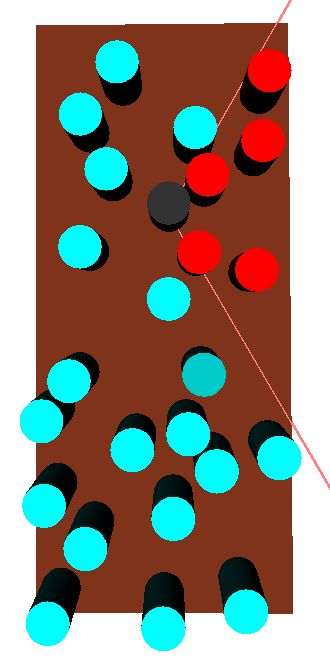
\includegraphics[scale=0.3,angle=90]{images/feature_cone.png}
  \caption{\small{If the target object to be grasped is the black can, we consider the objects
whose centers lie in a cone from angles $-\frac{\pi}{3}$ to $\frac{\pi}{3}$ toward the closest table edge in
our feature computations. These objects are shown here in red.}}
  \label{fig:cone}
\end{figure}

We now describe the feature vector $f(n)$ associated with a high-level plan. Because the plan is composed
of a sequence of object grasp and putdown actions, we first consider features of a single grasp action, targeted
at an object $o$ in the environment. Consider a cone ranging from angles $-\frac{\pi}{3}$ to $\frac{\pi}{3}$
toward the closest table edge from $o$, as shown in \figref{fig:cone}. The first feature, exists\_obstr, is a binary variable indicating
whether any other objects lie in this cone. The second, exists\_path, is a binary variable indicating whether there is a linear
grasp path wide enough for the robot's gripper to fit through within the cone. For the third feature, we approximate the robot's arm and gripper with a cylinder $c$ and sweep it across 10 discretized angles from $-\frac{\pi}{3}$ to
$\frac{\pi}{3}$. We then store the minimum number of collisions with $c$ as the feature, sweep\_count. This gives us a coarse approximation for the minimum number of object that should be moved before the target object is accessible via a linear path.
We construct these features for the first five grasp actions in the plan (padding with -1 if there are not enough).
We then add on the following aggregate features associated with the entire plan: 1) the minimum exists\_obstr across all grasp actions,
2) the sum of sweep\_count across all grasp actions, 3) the number of times $n$ was picked for refinement,
and 4) the number of times $n$ was picked for generating an error.
